\documentclass[12pt]{article}
\usepackage{preamble}

\pagestyle{fancy}
\fancyhead[LO,LE]{Физические основы компьютерных \\ и сетевых технологий}
\fancyhead[CO,CE]{07.10.2024}
\fancyhead[RO,RE]{Лекции Музыченко Я. Б.}

\fancyfoot[L]{\scriptsize исходники найдутся тут: \\ \url{https://github.com/pelmesh619/itmo_conspects} \Cat}

\begin{document}
    \section{5. Вращательное движение. Моменты силы и импульса}

    \begin{minipage}{\textwidth}
        \begin{wrapfigure}{r}{0pt}
            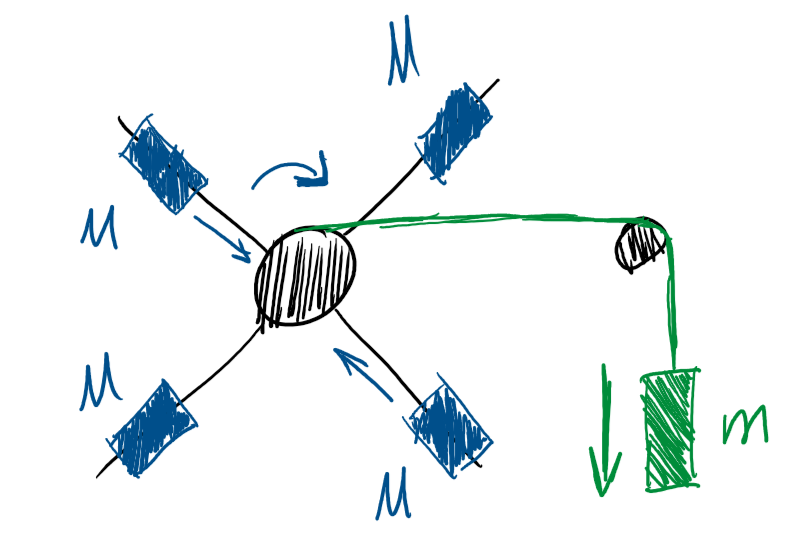
\includegraphics[height=5.5cm]{physics1/images/physics1_2024_10_07_1}
        \end{wrapfigure}

        Одной из лабораторный работ в курсе механики является работа с маятником Обербека (представлен на рисунке).
        Принцип его работы таков: к вращающемуся колесу с грузиками на спицах привязана нить, другой конец которой
        привязан к грузу через блок, груз падает, вращает колесо. В ходе эксперимента можно заметить, что при приближении
        грузиков к центру колесо начинает раскручиваться быстрее.

    \end{minipage}

    \mediumvspace

    Рассмотрим величины, действующие при вращательном движении:

    \smallvspace

    \begin{enumerate}

        \begin{minipage}{\textwidth}
            \begin{wrapfigure}{r}{0pt}
                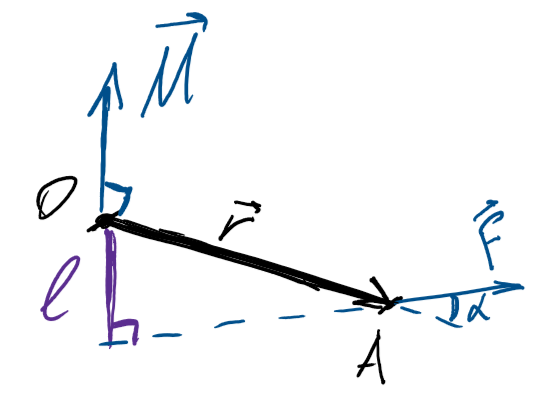
\includegraphics[width=0.3\textwidth]{physics1/images/physics1_2024_10_07_2}
            \end{wrapfigure}

            \item Момент силы $M$

            $M = F \cdot l$

            $\vec{M} = [\vec{r} \vec{F}] \qquad M = r \cdot F \cdot \sin\alpha = l \cdot F$

            Так как момент силы - векторное произведение, то вектор момента силы направлен перпендикулярно к плоскости
            радиус-вектора и вектора силы

            $[M] = \text{Н} \cdot \text{м}$

            % /з

            Аналогично рассмотрим момент силы для противоположных сил:

            \begin{wrapfigure}{r}{0pt}
                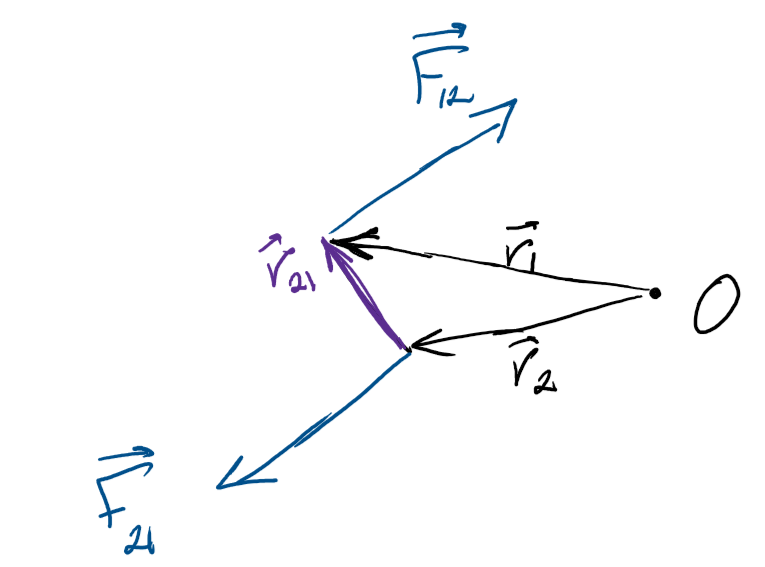
\includegraphics[width=0.3\textwidth]{physics1/images/physics1_2024_10_07_3}
            \end{wrapfigure}

            \item Момент пары сил

            $\vec{M} = \vec{M}_1 + \vec{M}_2 = [\vec{r}_1 \vec{F}_{12}] + [\vec{r}_2 \vec{F}_{21}] =
            [(\vec{r}_2 + \vec{r}_{21}) \vec{F}_{12}] + [\vec{r}_2 \vec{F}_{21}] = [\vec{r}_2 \vec{F}_{12}] + [\vec{r}_{21} \vec{F}_{12}] + [\vec{r}_2 \vec{F}_{21}]$

            $\vec{M} = [\vec{r}_{21} \vec{F}_{12}] = [\vec{r}_{12} \vec{F}_{21}]$

            Момент пары сил равен произведению вектора силы на радиус-вектор между точками приложения сил

            \begin{wrapfigure}{r}{0pt}
                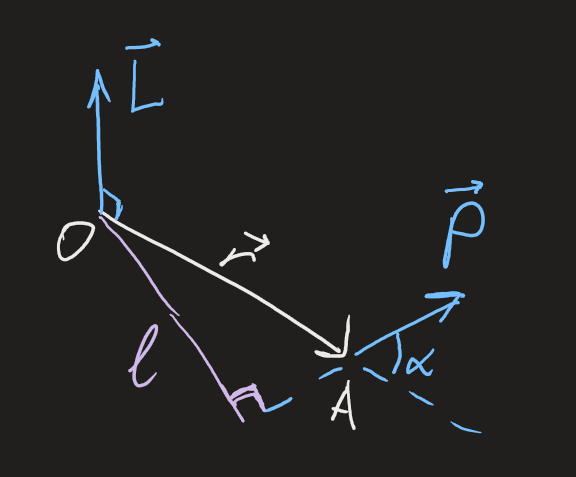
\includegraphics[width=0.3\textwidth]{physics1/images/physics1_2024_10_07_4}
            \end{wrapfigure}

            \item Момент импульса $L$

            Аналогично моменту силы можем определить момент импульса:

            $\vec{L} = [\vec{r} \vec{p}]$
            
            $L = r \cdot p \cdot \sin\alpha = p \cdot l$
            
            $[L] = \text{кг} \frac{\text{м}^2}{\text{с}} = \text{Н} \cdot \text{с} \cdot \text{м}$

            \item Уравнение моментов

            $\frac{d\vec{L}}{dt} = [\frac{d\vec{r}}{dt}\vec{p}] + [\vec{r} \frac{d\vec{p}}{dt}] = \cancelto{0}{[\vec{v} \vec{p}]} + [\vec{r} \vec{F}] = \vec{M}$ \hfill $\cancelto{0}{[\vec{v} \vec{p}]} \Longleftarrow \vec{v} \uparrow\uparrow \vec{p}$

            \fbox{$\frac{d\vec{L}}{dt} = \vec{M}$}
        \end{minipage}

        \smallvspace

        $\frac{d\vec{p}}{dt} = \vec{F} \quad \Longrightarrow \quad \vec{F}_\text{внешн} = 0 \Longrightarrow \vec{p} = const$ - закон сохранения импульса

        \smallvspace

        \begin{minipage}{\textwidth}
            \begin{wrapfigure}{r}{0pt}
                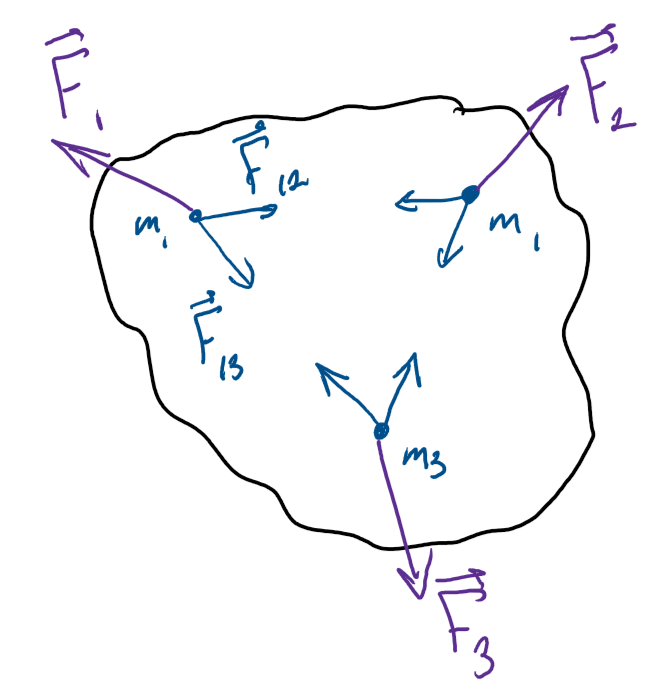
\includegraphics[width=0.3\textwidth]{physics1/images/physics1_2024_10_07_5}
            \end{wrapfigure}

            \item Закон сохранения момента импульса

            Пусть дана система материальных точек. На них действуют силы, которые мы можен разделить на внутренние и внешние

            В замкнутой системе внешние силы сведены к 0:

            $\frac{d\vec{L}}{dt} = \vec{M} = \vec{M}_{\text{внешн}} + \cancelto{0}{\vec{M}_{\text{внутр}}}$

            Поэтому:

            $\vec{M}_\text{внешн} = 0 \Longrightarrow \vec{L} = const$ - закон сохранения момента импульса

            \item Основное уравнение динамики вращательного движения

            $L_i = m_i v_i \cdot r_i = m_i \omega \cdot r_i^2 = \omega m_i r_i^2$
        \end{minipage}

        \smallvspace

        \begin{minipage}{\textwidth}
            \begin{wrapfigure}{r}{0pt}
                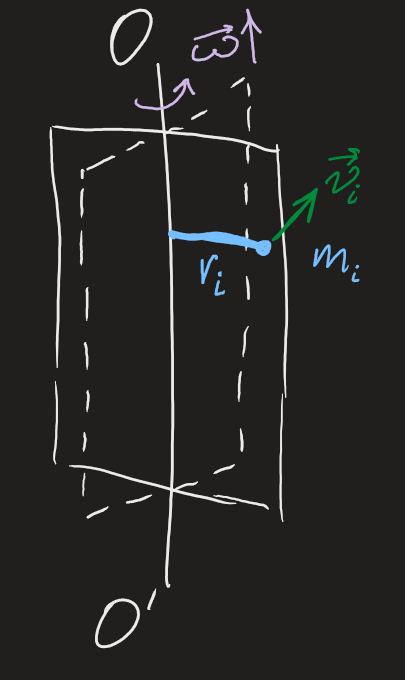
\includegraphics[width=0.2\textwidth]{physics1/images/physics1_2024_10_07_6}
            \end{wrapfigure}


            $L = \sum L_i = \omega \sum m_i r_i^2$

            $\vec{p} = m \vec{v} \qquad L_z = I \omega_z$

            $I = \sum m_i r_i^2$ - момент инерции системы материальных точек, $[I] = \text{с} \cdot \text{м}^2$

            В интегральной форме: $I = \int r^2 dm$

            Здесь же выделим различное распределение массы
        \end{minipage}

        \smallvspace
        
        \begin{enumerate}[label=\alph*) ]
            \item Линейное: $\tau = \frac{dm}{dl} = \frac{m}{l}$

            \item Поверхностное: $\sigma = \frac{m}{s} = \frac{dm}{ds}$

            \item Объемное: $\rho = \frac{m}{V} = \frac{dm}{dV}$
        \end{enumerate}

        $L_z = I \omega_z$

        $\frac{dL_z}{dt} = I \frac{d\omega_z}{dt} = I \beta_z$

        \fbox{$M_z = I \beta_z$} - основное уравнение динамики вращательного движения

        \item Расчет моментов инерции твердых тел

        Рассмотрим моменты инерции для твердых тел разной формы:

        \smallvspace
            
        \begin{enumerate}
            \begin{minipage}{0.95\textwidth}
                \begin{wrapfigure}{r}{0pt}
                    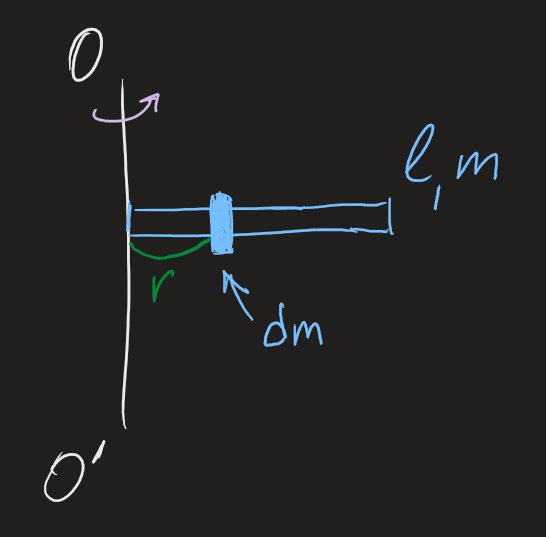
\includegraphics[width=0.2\textwidth]{physics1/images/physics1_2024_10_07_7}
                \end{wrapfigure}


                \item \textbf{Стержень}

                $I = \int r^2 dm$

                $I_{\text{м.т.}} = mr^2$

                $dI = r^2 \dm$

                $I = \sum_{i} d I_i = \int_0^l dI = \int_0^l r^2 dm = \int_0^l r^2 \tau dl = \int_0^l r^2 \tau dr = \tau \frac{r^3}{3} \Big|_0^l = \tau \frac{l^3}{3} = \frac{ml^2}{3}$

                \fbox{$I_\text{стерж} = \frac{ml^2}{3}$}

            \end{minipage}

            \begin{minipage}{0.95\textwidth}
                \begin{wrapfigure}{r}{0pt}
                    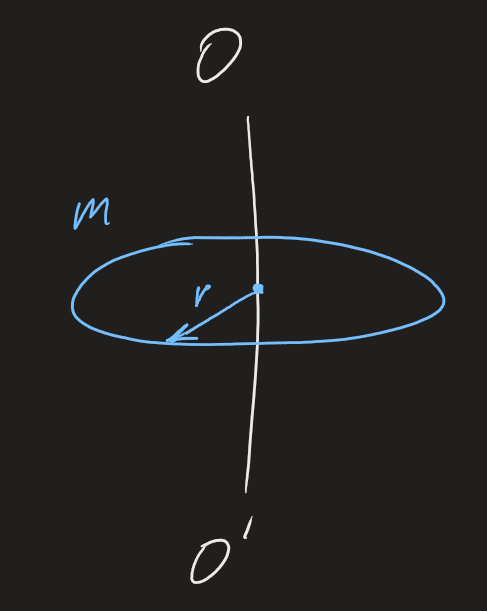
\includegraphics[width=0.2\textwidth]{physics1/images/physics1_2024_10_07_8}
                \end{wrapfigure}

                \item \textbf{Кольцо}

                Для кольца тривиально: \fbox{$I_\text{кольц} = r^2 m$}
                
                \item \textbf{Диск}

                Разбиваем диск на кольца с радиусом $r$ толщиной $dr$

                $dI = dm r^2 = \sigma ds r^2 = \sigma 2\pi r dr r^2 = \sigma ds r^2$

                $I = \int \sigma 2\pi r^3 dr = \sigma 2\pi \frac{R^4}{4} = \frac{mR^2}{2}$

                \fbox{$I_\text{диск} = \frac{mR^2}{2}$}

            \end{minipage}

            \begin{minipage}{0.95\textwidth}
                \begin{wrapfigure}{r}{0pt}
                    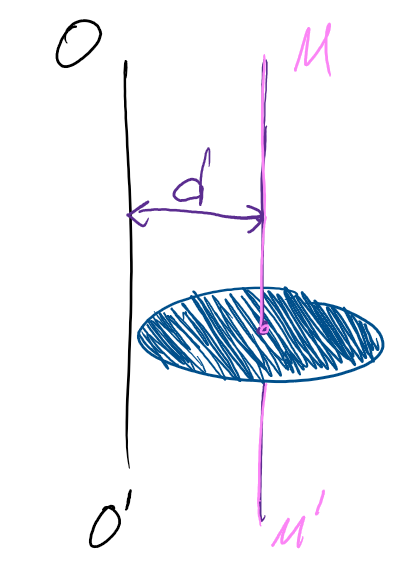
\includegraphics[width=0.2\textwidth]{physics1/images/physics1_2024_10_07_9}
                \end{wrapfigure}

                \item \textbf{Теорема Штейнера}

                Теорема Штейнера гласит, что момент инерции тела для неподвижной оси равен сумме момента инерции для оси тела, проходящей через центр масс и параллельной исходной и произведению квадрата расстояния и массы

                $I = I_0 + md^2$

                Пример: кольцо вращается вокруг оси, расположенной на торце кольца, зная момент импульса в центральной оси кольца 
                и расстояние между осями, можем узнать момент импульса для кольца

            \end{minipage}
        \end{enumerate}


    \end{enumerate}

\end{document}
